\documentclass{beamer}
\usepackage{ngerman}
\usepackage[utf8]{inputenc}
\usepackage{tikz}

% Auswahl des Designs
\usetheme{Warsaw}               

% Angaben zum Vortrag
\title[Short Title]{Full Title}
\author{Author}
\institute[Heidelberg University]{Heidelberg University}
\date[13.01.2023]{Seminar Mathematical Machine Learning \\ Fall 2022 \\ 13.01.2023}

\begin{document}

\begin{frame}
  \titlepage
\end{frame}

\begin{frame}
  \frametitle{Overview}
  \tableofcontents
\end{frame}


%---------------------------------------------------
\section{Introduction}
%---------------------------------------------------

\begin{frame}
  \frametitle{A Simple Slide}
  \begin{block}{Headline}
		Content of block
  \end{block}
  \begin{block}<2->{This block \ldots}
		only appears in the second frame.
  \end{block}
\end{frame}

\begin{frame}
  \frametitle{Another Slide}
  \begin{theorem}[Stability Function]
		The stability function of a Runge-Kutta method is given by
    \begin{equation*}
      R(z) = 1 + z \, c^\top (I-z \, B)^{-1} \vec{1}.
    \end{equation*}
  \end{theorem}
\end{frame}


%---------------------------------------------------
\section{Main Part}
%---------------------------------------------------

\begin{frame}
  \frametitle{Overview Repeated}
  \tableofcontents[currentsection]
\end{frame}

\begin{frame}
  \frametitle{A Slide in the New Section}
	\begin{block}{A figure produced using \texttt{tikz}}
    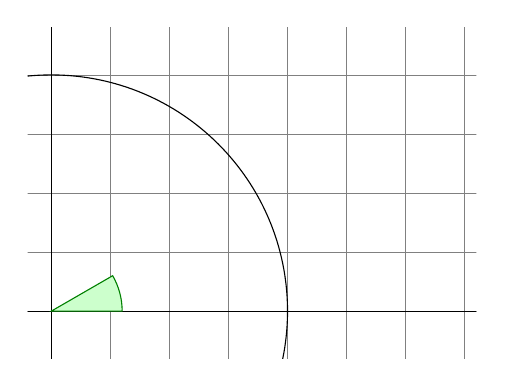
\begin{tikzpicture}[scale=3]
      \clip (-0.1,-0.2)
      rectangle (1.8,1.2);
      \draw[step=.25cm,gray,very thin]
      (-1.4,-1.4) grid (3.4,3.4);
      \draw (-1.5,0) -- (2.5,0);
      \draw (0,-1.5) -- (0,1.5);
      \draw (0,0) circle (1cm);
      \filldraw[fill=green!20!white,
      draw=green!50!black]
      (0,0) -- (3mm,0mm)
      arc (0:30:3mm) -- cycle;
    \end{tikzpicture}
  \end{block}
\end{frame}


\end{document}

